\documentclass[a4paper,12pt]{article}
% define the title

\author{Willem~Frishert}
\title{Shader~Labs}

\usepackage{subfigure}
\usepackage{graphicx}
\DeclareGraphicsRule{.JPG}{eps}{*}{`jpeg2ps #1} 

\newenvironment{mylisting}
{\begin{list}{}{\setlength{\leftmargin}{1em}}\item\scriptsize\bfseries}
{\end{list}}

\newenvironment{mytinylisting}
{\begin{list}{}{\setlength{\leftmargin}{1em}}\item\tiny\bfseries}
{\end{list}}

\begin{document}
\pagestyle{headings}
% generates the title
\maketitle

\section{Introduction}
\label{sec:Introduction}
This document contains a brief description of different shader effects and the algorithms used to implement them. The shaders have been made for the lab of the real-time rendering course and have been implemented in the GLSL (OpenGL Shading Language). The lab requires implementing two shaders (single pass rendering) and one multi-pass image filter (at least three passes supported). The choice was made to do a a phong shader, a toon shader and a bloom shader as a multi-pass image filter.

\section{Phong Shader}
\label{sec:PhongShader}
\subsection{Description}
\label{sec:Description}

There are two types of shading that OpenGL supports by default. These are flat shading and Gouraud shading. Flat shading gives a polygon one single color whereas Gouraud shading uses normals per vertices to calculate the intensity per vertex and then interpolates the intensity along the polygon. The latter type of shading works well for diffuse surfaces but specular highlights are not shown correctly. To correctly deal with specular highlights, Phong shading should be used. Instead of calculating the intensity per vertex and interpolating this intensity along the polygon, the normal of each vertex is interpolated along the polygon. After this is achieved the intensity per fragment is calculated based on the vertex normal, the view direction and the light direction.


\subsection{Implementation}
\label{sec:ImplementationPhongShader}

The phong shader is a single pass rendering algorithm, consisting of a vertex and fragment shader. The vertex shader task is to calculate the normal per vertex and calculate the view vector per vertex. Both these vectors are then interpolated over the triangle and handled by the fragment shader.

The fragment shader receives the interpolated normal and view direction vector and then calculates the ambient, diffuse and specular component using the vertex normal, the view direction vector and the lighting direction vector. In this calculation, the angle between the normal vector and light vector (dot product) is used to for the diffuse component. For the specular component, the reflection vector is calculated using:

	\[ reflection = light-2 \times (normal \cdot light) \times normal \]

Where after, the angle between the reflection vector and the view vector (another dot product) is calculated. The shininess of the material is then used to calculate the sharpness of the lobe.

\subsection{Pitfalls}
\label{sec:PitfallsPhongShader}

There are not that many pitfalls during the implementation of this shader; however, to calculate the reflection vector, the direction of the light has to point towards the surface.

%\pagebreak[4]

\begin{figure}[htbp]
  \begin{center}
    \mbox{
      \subfigure[gouraud shading] {\scalebox{0.4} {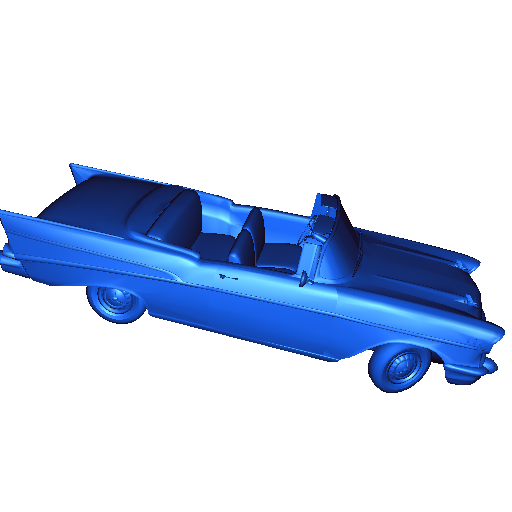
\includegraphics[width=512px]{images/gouraud.png}}} \quad
      \subfigure[phong shading]   {\scalebox{0.4} {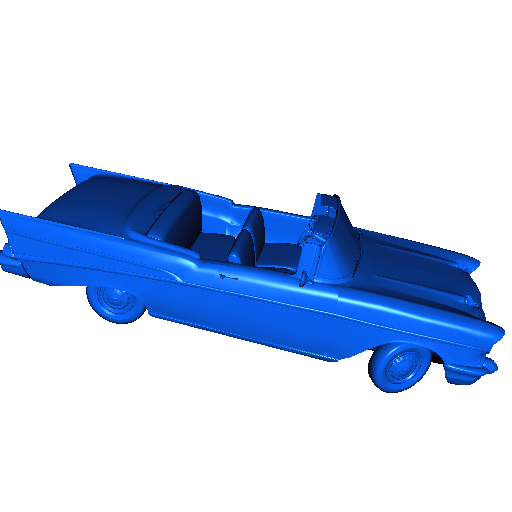
\includegraphics[width=512px]{images/phong.png}}}
      }
    \caption{gouraud versus phong shading}
    \label{fig:phongShading}
  \end{center}
\end{figure}

%\begin{figure}
%	\centering
%		\mbox{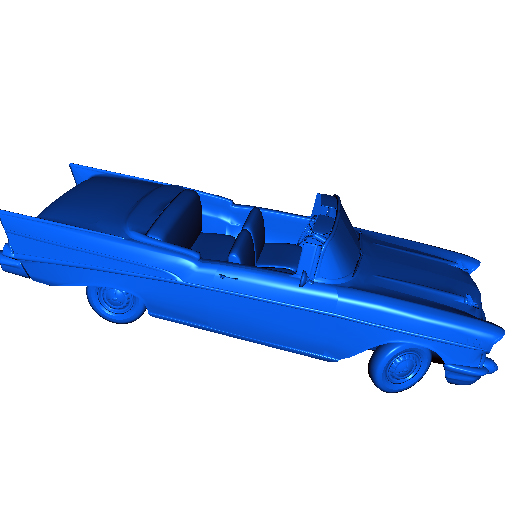
\includegraphics[width=128px]{images/phong.jpg}}
%	\caption{Phong Shading}
%	\label{fig:phongShading}
%\end{figure}

%\mbox{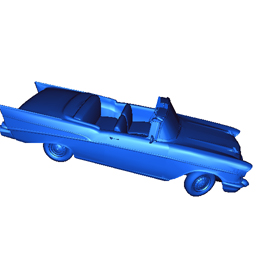
\includegraphics[width=256px, bb= 0 0 256 256]{images/gouraud.jpg}}

\subsection{Phong shader result}
\label{sec:PhongShaderResult}
Figure~\ref{fig:phongShading} shows the the result of the phong shader in comparison with gouraud shading done by OpenGL.


\section{Toon Shader}
\label{sec:ToonShader}
\subsection{Description}
\label{sec:DescriptionToonShader}

The idea of a toon shader is to use a 3D rendering technique that is used to simulate the 2D style of cartoons. This type of non-photorealistic rendering is also known as cel-shading where only a few different levels of intensities are specified. Therefore the model will end up with only a few different shades across the surface.

\subsection{Implementation}
\label{sec:ImplementationToonShader}

There are several different ways to implement a toon shader but share the same basic idea. In the vertex shader the vertex normal is rotated accordingly and interpolated across the triangle. In the fragment shader, the appropriate intensity is picked based on the angle between the light direction and the normal (dot-product). Several methods online describe the use of a lookup table in the form of a texture (See Figure~\ref{fig:TextureLUT}). The idea is that the texture only contains a number intensities and uses nearest neighbor when being accessed. Thus the dot-product is used as an index to get the intensity from the texture and no conditional control flow has to be implemented. Every fragment will execute the same code and be done at (roughly) the same time.

\begin{figure}[h]
  \begin{center}
		\scalebox{0.5} {
\includegraphics[width=512px]{images/lightmap.png}}
    \caption{An example of a texture lookup table.}
    \label{fig:TextureLUT}
  \end{center}
\end{figure}


One additional step that can easily be implemented is to give the object a black edge which makes it look like it's really a cartoon. A way to obtain this is to render the object's backside (front face culling) with the polygon mode set to lines. During this step, the toon shader is disabled and the line width is set to a higher value than the default. On top of this, the front side is rendered with the toon shader on.

\subsection{Pitfalls}
\label{sec:PitfallsToonShader}

One of the troubles during implementation was the fact that the texture (the lookup table) was linearly interpolated by OpenGL and thus the result did not look accurate as expected. It took quite a while to discover that this was the problem since the texture at this point was also set to repeat and thus the first and last pixel in the texture were also interpolated which gave a strange effect

%\pagebreak[4]

\begin{figure}[htbp]
  \begin{center}
		\scalebox{0.5} {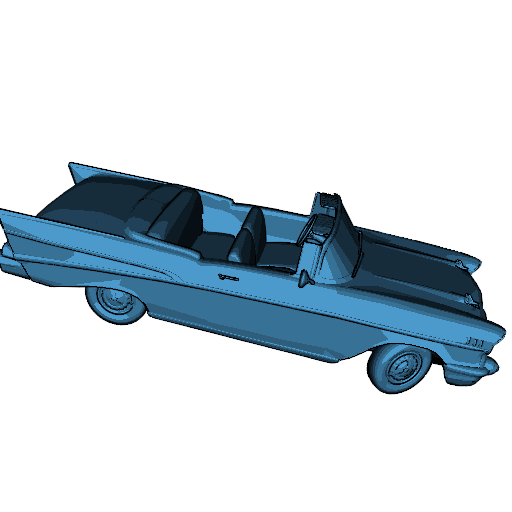
\includegraphics[width=512px]{images/toon.png}}
    \caption{toon shading}
    \label{fig:toonShading}
  \end{center}
\end{figure}

\subsection{Toon shader result}
\label{sec:ToonShaderResult}

Figure~\ref{fig:toonShading} shows the the result of the toon shader. In total, there are 7 different levels being used to generate this effect.

\section{Bloom Shader}
\label{sec:BloomShader}

\subsection{Description}
\label{sec:DescriptionBloomShader}

The bloom effect allows bright highlights to be perceived as even brighter on screen while darkened areas remain similar. To achieve this result, multi-pass image filtering has to be executed in order to extract the right information from the images and combine several of them to form the final image.

To obtain the images, a technique is used which allows to extract images from the frame buffer. Using this method, images are generated and can be used as input for the next pass


\subsection{Implementation}
\label{sec:ImplementationBloomShader}

The OpenGL frame buffer objects (FBOs) allow to the generated image to be rendered to a texture. It gives the program the ability to write to the frame buffer as if it would to display. However, instead of writing to display, the pixels are being put on a texture. After generating this texture, is it connected to screen size quad, oriented perpendicular to the screen in order to use for the next pass. Every time a pass is done, a different shader program (filter) is enabled to obtain a new texture. Below an image is showing the different textures which are generated through each pass and as can be seen, the original image, together with three levels of blur are combined to form an image on the display. Each pass will now be discussed separately.

\subsubsection{Generating original image}
\label{sec:GeneratingOriginalImage}

The first pass is generating the original texture. For this, the phong shader that was described earlier, is used (see section~\ref{sec:PhongShader} on page~\pageref{sec:PhongShader}). The pass uses the phong vertex and fragment shader. However, this could easily be any other input.

\subsubsection{Extracting the bright spots}
\label{sec:ExtractingTheBrightSpots}
The second pass is to extract the bright spots in the scene. This is done using a filter which takes the original texture and writes to a new texture, the bright pass texture. The filter is a shader program consisting of a single fragment shader. The fragment shader retrieves a value of the texture map and with the use of a sigmoidal function (also known as smoothstep function in GLSL terminology), a new intensity is calculated which is then put on to the bright pass texture. Note that the new intensity is calculated per color component instead of looking at the components in total.

\subsubsection{Blurring}
\label{sec:Blurring}
The next six passes create three different levels of blurred textures. To create a nice effect, Gaussian blur is used with a kernel of a certain size. Since the kernel is circularly symmetric, the Gaussian blur can be applied to a two-dimensional image as two independent one-dimensional calculations. This means that, instead of having \[O(m \times n \times M \times N)\] the performance will increase since the calculation is done in \[ O(m \times M \times N) + O(n \times M \times N) \] In order to linearly separate the Gaussian kernel into a horizontal direction blur and on top of that a vertical direction blur a two pass filter are used to create a single blurred texture.
Another problem which occurs when blurring with a Gaussian kernel is that, if the sample points are taken too far apart from each other, a "ghosting" effect occurs. The resolution to this problem is to apply a small kernel multiple times to several blurred images and then adding the blurred textures together. The implementation of this effect is done in a fragment shader. The fragment shader uses a 7 sample points and contains a boolean to specify whether the kernel should be aligned vertically of horizontally. Using a two pass generates a 7*7 Gaussian kernel.

\subsubsection{Combining the textures}
\label{sec:CombiningTheTextures}

The final pass is to combine the original images together with the blurred textures. This means that all four textures are added to a screen perpendicular quad (using multi-texturing) and a fragment shader is enabled to combine all for four textures.

\subsection{Pitfalls}
\label{sec:PitfallsBloomShader}
The trouble with multi-pass image filtering is that there are lot of different components involved. Each shader has to run at the correct time with the correct textures and variables as input. This makes it quite confusing and good structure of code is essential. Unfortunately, then it is still quite hard to debug the code. One way is to output the textures seperately to screen to see in which pass a problem occurs.

%\pagebreak[4]
\begin{figure}[ht]
  \begin{center}
    \mbox{
      \subfigure[phong shading] {\scalebox{0.2} {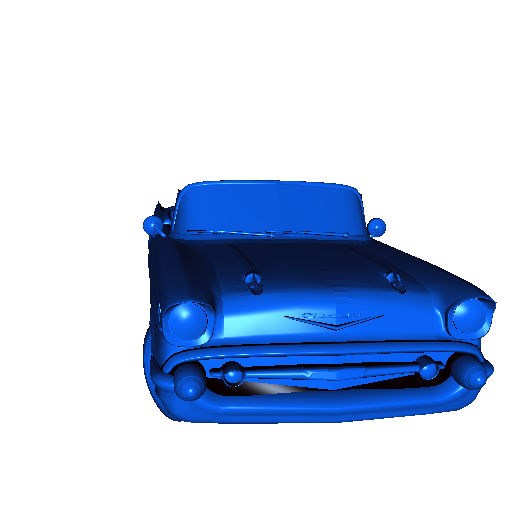
\includegraphics[width=512px]{images/phong2.png}}} \quad
      \subfigure[brightpass]    {\scalebox{0.2} {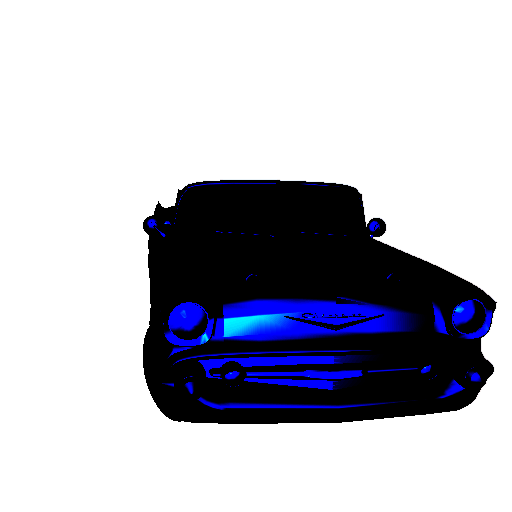
\includegraphics[width=512px]{images/brightpass.png}}} \quad
      \subfigure[first blur]    {\scalebox{0.2} {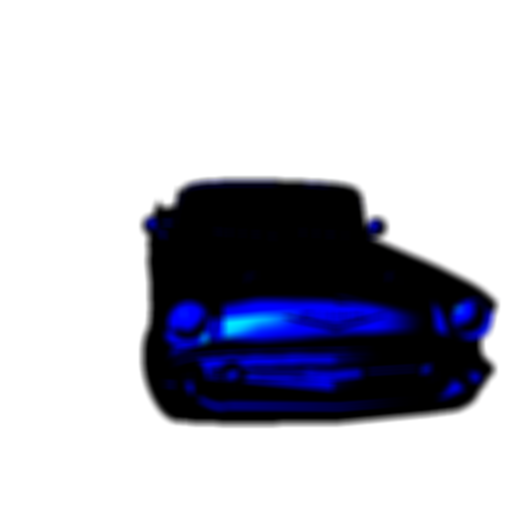
\includegraphics[width=512px]{images/firstblur.png}}} \quad
      }
    \mbox{
      \subfigure[second blur]   {\scalebox{0.2} {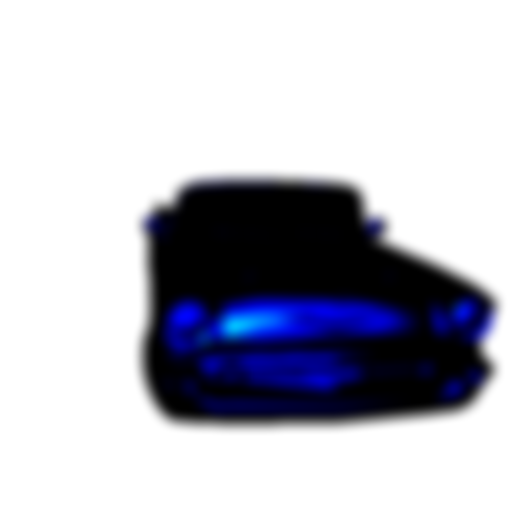
\includegraphics[width=512px]{images/secondblur.png}}} \quad
      \subfigure[third blur]    {\scalebox{0.2} {
\includegraphics[width=512px]{images/thirdblur.png}}} \quad
      \subfigure[final image]   {\scalebox{0.2} {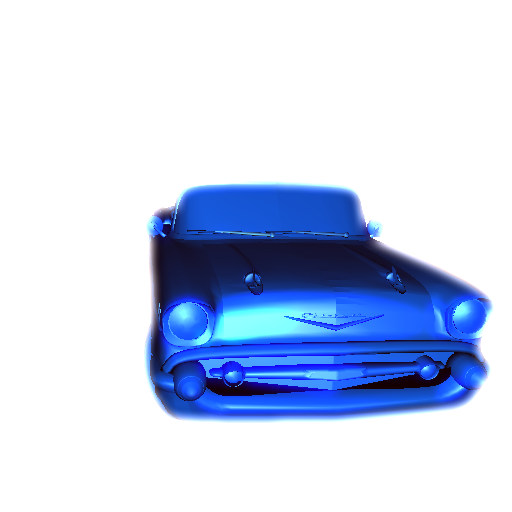
\includegraphics[width=512px]{images/bloom.png}}}
      }
    \caption{phong shading and the blooming effect applied to it}
    \label{fig:bloomPassShading}
  \end{center}
\end{figure}

\subsection{Bloom shader result}
\label{sec:bloomShaderResult}
Figure~\ref{fig:bloomPassShading} shows the different textures obtained during the passes. The phong shaded image is used as original image and combined with the three different blurred textures to form the final image

\section{Conclusion}
\label{sec:Conclusion}
Building shaders can be tricky since it requires the programmer to think in vertices and fragments instead of meshes and scenes. It's good to start building a simple shader like the phong shader and from there on up work your way to something more complicated like the multi-pass filtering. Of course the pitfalls, such as whether to normalize a vector or not, will still be there. The only way to debug problems is to output pieces of information to the screen and check if they are correct, which is half the fun of the job.

\begin{thebibliography}{99}
	\bibitem{lighthouse3d.com} lighthouse3d.com: \emph{GLSL Tutorial}, www.lighthouse3d.com (2006)
	\bibitem{OpenGLShadingLanguage} R.J. Rost, \emph{OpenGL Shading Language}, 2nd Edition (2006)
	\bibitem{3DComputerGraphics} A.H. Watt: \emph{3D Computer Graphics}, 3rd Edition (2000)
	\bibitem{Cel-shading} S. Hamlaoui: \emph{Cel-shading}, www.gamedev.net
	\bibitem{HowtodogoodbloomforHDRrendering} H. Kalogirou: \emph{How to do good bloom for HDR rendering}, harkal.sylphis3d.com (2006)
\end{thebibliography}

\pagebreak[4]

\section{Source code shaders}
\label{sec:SourceCodeShaders}

\paragraph{Phong shader}
\label{sec:PhongShaderSource}


\begin{mylisting}
	\begin{verbatim}
/*!
 * phong.vert
 * 
 * Willem Frishert
 */

varying vec3 vNormal; //normal at vertex
varying vec3 vView; // view vector towards vertex

void main(void)
{
  //calculate the normal per vertex and have it interpolated.
  vNormal = gl_NormalMatrix * gl_Normal;

  //calculate the view vector and have it interpolated.
  vView = vec3(gl_ModelViewMatrix * gl_Vertex);
  
  //3d Screen space:
  //These two instructions are pretty much the same. ftransform is more precise though.
  //gl_Position = gl_ModelViewProjectionMatrix * gl_Vertex;
  gl_Position = ftransform();
}


/*!
 * phong.frag
 * 
 * Willem Frishert
 */


uniform float Ka; //(0.0-1.0)
uniform float Ks; //(0.0-1.0)
uniform float Kd; //(0.0-1.0)

varying vec3 vNormal;  //interpolated normal accross the polygon
varying vec3 vView; //interpolated view vector

void main(void)
{
  vec3 normalVector  = normalize(vNormal);
  vec3 viewVector    = normalize(vView);
  vec3 reflectVector = reflect( gl_LightSource[0].position.xyz, normalVector ); 

  vec4 intensityAmbient  = vec4(Ka) * gl_FrontMaterial.ambient  * gl_LightSource[0].ambient;
  vec4 intensityDiffuse  = vec4(Kd) * gl_FrontMaterial.diffuse
                             * gl_LightSource[0].diffuse
                             * clamp( dot( normalVector, gl_LightSource[0].position.xyz ), 0.0, 1.0 );
                                    
  vec4 intensitySpecular = vec4(Ks) * gl_FrontMaterial.specular 
                             * gl_LightSource[0].specular
                             * pow( clamp( dot( reflectVector, viewVector ), 0.0, 1.0 ),
                                    gl_FrontMaterial.shininess );

  gl_FragColor = intensityAmbient + intensityDiffuse + intensitySpecular;
}

	\end{verbatim}
\end{mylisting}

\pagebreak[4]

\paragraph{Toon shader}
\label{sec:ToonShaderSource}


\begin{mylisting}
	\begin{verbatim}
/*!
 * toontexture.vert
 * 
 * Willem Frishert
 */

varying vec3 vNormal;

void main()
{
  vNormal = normalize(gl_NormalMatrix * gl_Normal);
		
  gl_Position = ftransform();
}





/*!
 * toontexture.frag
 * 
 * Willem Frishert
 */

uniform sampler2D lightMap;
uniform float red, green, blue;
varying vec3 vNormal;

void main()
{
  vec3 vNormalized = normalize(vNormal);

  // calculate angle between light and surface normal
  float dotLN = clamp( dot( gl_LightSource[0].position.xyz, vNormalized ), 0.0, 1.0 );

  // use dot-product as index for lookup table
  vec4 intensity = texture2D( lightMap, vec2( dotLN, 0.0 ) );	

  gl_FragColor = vec4( intensity.r * red, 
                       intensity.g * green,
                       intensity.b * blue,
                       1.0 );
}
	\end{verbatim}
\end{mylisting}


\pagebreak[4]

\paragraph{Bloom shader}
\label{sec:BloomShaderSource}
\begin{mylisting}
	\begin{verbatim}
/*!
 * brightpass.frag
 * 
 * Willem Frishert
 */

uniform sampler2D textureMap;
uniform float thresholdBrightness;

void main(void)
{
  vec4 texel = texture2D( textureMap, gl_TexCoord[0].st );
	
  // calculate the new intensity using a sigmoidal function (smoothstep)
  vec3 newIntensity = smoothstep( vec3( thresholdBrightness ),
                                  vec3(1.0), texel.rgb );

  gl_FragColor = vec4( newIntensity , texel.a );
}




/*!
 * blureffect.frag
 * 
 * Willem Frishert
 */

uniform float sampleDistance;
uniform sampler2D textureMap;
uniform bool horizontalBlur;

const int KNumberOfSamples = 13;

void main(void)
{
  // either horizontal blur or vertical blur
  vec2 blurType = vec2( float(horizontalBlur), float(!horizontalBlur) );
  vec4 sum = vec4 ( 0.0 );

  vec2 samples[KNumberOfSamples];
  samples[0]  = vec2( -0.6 );
  samples[1]  = vec2( -0.5 );
  samples[2]  = vec2( -0.4 );
  samples[3]  = vec2( -0.3 );
  samples[4]  = vec2( -0.2 );
  samples[5]  = vec2( -0.1 );
  samples[6]  = vec2(  0.0 ); // actual location
  samples[7]  = vec2(  0.1 );
  samples[8]  = vec2(  0.2 );
  samples[9]  = vec2(  0.3 );
  samples[10] = vec2(  0.4 );
  samples[11] = vec2(  0.5 );
  samples[12] = vec2(  0.6 );

  for (int i = 0; i < KNumberOfSamples; i++)
  {
    sum += texture2D( textureMap, gl_TexCoord[0].st 
            + sampleDistance * (samples[i] * blurType) );
  }

  sum /= float(KNumberOfSamples);
  gl_FragColor = vec4( sum );
}




/*!
 * combine.frag
 * 
 * Willem Frishert
 */


uniform sampler2D originalTexture;
uniform sampler2D blurTexture1;
uniform sampler2D blurTexture2;
uniform sampler2D blurTexture3;

void main(void)
{
  vec4 sum = vec4(0.0);

  // get 4 textures and add them together
  sum += texture2D(originalTexture, gl_TexCoord[0].st);	
  sum += texture2D(blurTexture1, gl_TexCoord[0].st);	
  sum += texture2D(blurTexture2, gl_TexCoord[0].st);
  sum += texture2D(blurTexture3, gl_TexCoord[0].st);
		
  gl_FragColor = sum;		
} 
	\end{verbatim}
\end{mylisting}
\end{document}